% =============================================================================
% HEXACORE — Presentación de la Entrega
%
% Se compila con pdflatex desde esta carpeta (las rutas de los diagramas son
% relativas a ella):
%
%   latexmk -pdf Presentacion.tex
%
% El PDF resultante va a Documentation/Submission/, no aquí: en Work/ solo
% viven las fuentes.
% =============================================================================
% `xcolor={table}` habilita \rowcolor, que se usa para resaltar filas en las tablas
% densas (ASR de riesgo alto, ADR decididos con PoC, estado por integrante).
\documentclass[aspectratio=169,10pt,xcolor={table}]{beamer}

\usepackage[utf8]{inputenc}
\usepackage[T1]{fontenc}
\usepackage[spanish,es-noquoting,es-tabla]{babel}
\usepackage{booktabs}
\usepackage{array}
\usepackage{pifont}
\usepackage{pgfplots}
\usepackage{tikz}
\usepackage{xcolor}
\pgfplotsset{compat=1.18}
\usetikzlibrary{positioning, arrows.meta, shapes.geometric}

% --- Tema -------------------------------------------------------------------
\usetheme{metropolis}
\metroset{block=fill, sectionpage=progressbar, numbering=fraction, progressbar=frametitle}

% Paleta propia: azul profundo como color de marca, y tres semáforos que se
% usan en todo el documento para el estado de cada caso de uso.
\definecolor{hexazul}{HTML}{1B3A5C}
\definecolor{hexaacento}{HTML}{0E7C7B}
\definecolor{hexaok}{HTML}{1B7F3B}
\definecolor{hexaparcial}{HTML}{B8860B}
\definecolor{hexapend}{HTML}{8B1A1A}
\definecolor{hexagris}{HTML}{F2F4F6}

\setbeamercolor{frametitle}{bg=hexazul, fg=white}
\setbeamercolor{progress bar}{fg=hexaacento, bg=hexagris}
\setbeamercolor{title separator}{fg=hexaacento}
\setbeamercolor{alerted text}{fg=hexaacento}
\setbeamercolor{block title}{bg=hexagris, fg=hexazul}
\setbeamercolor{block body}{bg=hexagris!45}

% --- Marcas de estado -------------------------------------------------------
\newcommand{\ok}{\textcolor{hexaok}{\ding{51}}}
\newcommand{\parcial}{\textcolor{hexaparcial}{\ding{108}}}
\newcommand{\pend}{\textcolor{hexapend}{\ding{55}}}
\newcommand{\cifra}[1]{{\color{hexaacento}\textbf{#1}}}

% Márgenes laterales: metropolis deja 1 cm por lado; con tablas anchas se
% agradece recuperar ese espacio.
\setbeamersize{text margin left=0.7cm, text margin right=0.7cm}

% Los bloques traen un relleno vertical generoso que, sumado a una tabla,
% desborda la diapositiva.
\setbeamertemplate{block begin}{%
  \begin{beamercolorbox}[colsep*=0ex,dp=0.6ex,center]{block title}%
    \usebeamerfont{block title}\insertblocktitle%
  \end{beamercolorbox}%
  \nointerlineskip%
  \begin{beamercolorbox}[colsep*=0ex,vmode]{block body}%
    \vspace{0.4ex}\begin{minipage}{\textwidth-1ex}\hspace*{0.5ex}}
\setbeamertemplate{block end}{%
    \end{minipage}\vspace{0.6ex}%
  \end{beamercolorbox}\vspace{0.4ex}}

% Tablas más legibles en pantalla.
\renewcommand{\arraystretch}{1.08}
\newcolumntype{L}[1]{>{\raggedright\arraybackslash}p{#1}}
\newcolumntype{C}[1]{>{\centering\arraybackslash}p{#1}}

\title{Sistema Integral de Gestión de Eventos}
\subtitle{Arquitectura de Software · SRS, SAD y prototipo funcional}
\author{Daniel Cristancho \and Samuel Emperador \and Sebastián Sánchez \and Diego Coronado}
\institute{Pontificia Universidad Javeriana · HEXACORE}
\date{Septiembre de 2026}

\begin{document}

\maketitle

% =============================================================================
\begin{frame}{Qué vamos a ver}
  \setbeamertemplate{section in toc}[sections numbered]
  \footnotesize
  \begin{columns}[T]
    \begin{column}{0.5\textwidth}
      \tableofcontents[sections={1-5}]
    \end{column}
    \begin{column}{0.5\textwidth}
      \tableofcontents[sections={6-10}]
    \end{column}
  \end{columns}
\end{frame}

% =============================================================================
\section{Especificación de requisitos (SRS)}

\begin{frame}{El sistema en una frase}
  \begin{block}{Alcance}
    Gestiona el ciclo completo de un evento masivo ---conciertos, partidos, ferias---
    \textbf{desde la venta de entradas hasta la operación en campo} el día del evento.
  \end{block}

  \vspace{0.4em}
  \begin{columns}[T]
    \begin{column}{0.48\textwidth}
      \textbf{Seis frentes funcionales}
      \begin{itemize}\small
        \item Boletería y validación de QR
        \item Mercado secundario (reventa)
        \item Personal, turnos y logística
        \item Alimentos y bebidas
        \item Parqueaderos
        \item Administración y emergencias
      \end{itemize}
    \end{column}
    \begin{column}{0.48\textwidth}
      \textbf{Queda fuera}
      \begin{itemize}\small
        \item Procesamiento de pagos \textit{(pasarela externa)}
        \item Envío físico de notificaciones \textit{(proveedor externo)}
        \item Contabilidad de la organizadora
        \item Integración con venta de terceros
      \end{itemize}
    \end{column}
  \end{columns}

  \vspace{0.6em}
  \footnotesize
  El SRS dice \textbf{qué} debe hacer el sistema; el SAD, \textbf{cómo}. Por eso en el SRS no se
  nombra ningún motor de base de datos, lenguaje ni biblioteca: un requisito bien escrito
  sobrevive a un cambio de tecnología.
\end{frame}

\begin{frame}{Actores y las tres interfaces}
  \begin{columns}[T]
    \begin{column}{0.54\textwidth}
      \footnotesize
      \begin{tabular}{L{2.2cm}L{4.6cm}}
        \toprule
        \textbf{Actor} & \textbf{Qué hace} \\
        \midrule
        Cliente & Compra, revende, pide comida, reserva parqueadero \\
        Empleado & Turnos, asistencia, valida QR, reporta incidentes \\
        Organizador & Crea eventos, asigna personal, consulta reportes \\
        Administrador & Cuentas, roles, recintos, conciliación \\
        Supervisor & Activa y coordina la evacuación \\
        \midrule
        \textit{Pasarela de pagos} & \textit{Externo:} cobros y reembolsos \\
        \textit{Notificaciones} & \textit{Externo:} correo, push, SMS \\
        \bottomrule
      \end{tabular}
    \end{column}
    \begin{column}{0.44\textwidth}
      \textbf{Interfaces}
      \begin{itemize}\small
        \item \textbf{Portal web de clientes} --- cartelera, compra, reventa, cuenta.
        \item \textbf{Portal web administrativo} --- eventos, personal, recintos, reportes.
        \item \textbf{App móvil (Flutter)} --- la única que se usa \textit{dentro} del evento;
              sirve a Cliente y a Personal, y debe tolerar conectividad intermitente.
      \end{itemize}
      \vspace{0.3em}
      \footnotesize
      Un mismo usuario puede tener varios roles: quien trabaja en un evento también compra
      entradas para otro.
    \end{column}
  \end{columns}
\end{frame}

\begin{frame}{32 casos de uso en seis bloques}
  \footnotesize
  \begin{tabular}{L{3.4cm}C{2.1cm}L{7.2cm}}
    \toprule
    \textbf{Bloque} & \textbf{Casos de uso} & \textbf{Alcance} \\
    \midrule
    Boletería & CU-001 -- 005 & Consulta, compra, validación de QR, cancelaciones, promociones \\
    Mercado secundario y personal & CU-006 -- 010 & \textbf{Reventa segura (complejo)}, personal,
      turnos, asistencia, \textbf{evacuación (complejo)} \\
    Alimentos y bebidas & CU-011 -- 015 & Pedidos, menú e inventario, preparación, entrega por QR \\
    Logística y operación & CU-016 -- 020 & Planificación, personal operativo, monitoreo, incidentes \\
    Parqueaderos & CU-021 -- 025 & Reserva, ingreso/salida, espacios, cobro, ocupación \\
    Administración general & CU-026 -- 032 & Eventos, cuentas, roles, recintos, proveedores,
      pagos, reportes \\
    \bottomrule
  \end{tabular}

  \vspace{0.8em}
  \begin{alertblock}{Los dos casos complejos son el hilo conductor del SAD}
    \textbf{CU-006 (Mercado Secundario)} por la concurrencia sobre un recurso único, y
    \textbf{CU-010 (Evacuación)} por la entrega garantizada de instrucciones bajo presión de tiempo.
  \end{alertblock}
\end{frame}

\begin{frame}{Requisitos no funcionales con umbral verificable}
  \scriptsize
  \begin{tabular}{C{1.3cm}L{8.4cm}L{3.4cm}}
    \toprule
    \textbf{RNF} & \textbf{Enunciado} & \textbf{Atributo} \\
    \midrule
    RNF-01 & Ninguna entrada publicada puede venderse a dos compradores & Consistencia \\
    RNF-02 & Al transferirse, el QR anterior queda invalidado antes de emitir el nuevo & Consistencia \\
    RNF-03 & Sigue atendiendo ante la caída de una instancia de cualquier servicio & Disponibilidad \\
    RNF-04 & Ante una caída, se recupera sin intervención manual & Disponibilidad \\
    RNF-05 & Nunca almacena datos completos de tarjetas de pago & Seguridad \\
    RNF-06 & Toda petición pasa autenticada y autorizada por rol desde el Gateway & Seguridad \\
    RNF-07 & La consulta de disponibilidad responde con baja latencia en la apertura & Desempeño \\
    RNF-10 & El servicio de Entradas escala sin degradar los demás dominios & Escalabilidad \\
    RNF-11 & Toda operación financiera queda auditada & Trazabilidad \\
    RNF-15 & Una versión nueva se despliega sin interrumpir el servicio & Desplegabilidad \\
    RNF-17 & Al activarse una evacuación, todo el personal recibe su instrucción & Seguridad física \\
    RNF-18 & Cada microservicio puede probarse aislado, sin levantar los demás & Comprobabilidad \\
    \bottomrule
  \end{tabular}

  \vspace{0.6em}
  \footnotesize
  Son 18 en total. Cada uno fija una \textbf{métrica y un umbral}, no una intención: es lo que
  permite que la sección de atributos de calidad de esta presentación muestre números y no
  adjetivos.
\end{frame}

% =============================================================================
\section{Modelo de dominio}

\begin{frame}{Conceptos derivados de los 32 casos de uso}
  \scriptsize
  \begin{columns}[T]
    \begin{column}{0.5\textwidth}
      \begin{tabular}{L{2.1cm}L{4.4cm}}
        \toprule
        \textbf{Concepto} & \textbf{Qué es} \\
        \midrule
        Evento & Actividad con fecha, recinto, localidades y aforo \\
        Entrada & Boleto con QR único, ligado a su propietario actual \\
        Publicación de reventa & Oferta de una entrada ya adquirida \\
        Recinto / Zona & Lugar físico y sus subdivisiones con aforo \\
        Usuario / Cuenta & Persona registrada con sus roles \\
        Rol / Permiso & Acciones autorizadas sobre un módulo \\
        Personal & Trabajador con rol operativo \\
        Turno & Periodo de trabajo con horario y zona \\
        \bottomrule
      \end{tabular}
    \end{column}
    \begin{column}{0.5\textwidth}
      \begin{tabular}{L{2.3cm}L{4.2cm}}
        \toprule
        \textbf{Concepto} & \textbf{Qué es} \\
        \midrule
        Registro de asistencia & Marca de ingreso y salida en un turno \\
        Parqueadero / Espacio & Zona de estacionamiento y cada cupo \\
        Pedido & Solicitud de alimentos durante el evento \\
        Establecimiento & Punto de venta y su menú \\
        Pago & Transacción procesada por la pasarela externa \\
        Proveedor & Tercero contratado para la operación \\
        Incidente & Anomalía, hasta activar una evacuación \\
        Reporte & Consulta agregada para decidir \\
        \bottomrule
      \end{tabular}
    \end{column}
  \end{columns}

  \vspace{0.6em}
  \footnotesize
  \textbf{La decisión que atraviesa todo el modelo:} la \textbf{Entrada} tiene un solo
  propietario en cada momento y un QR que lo identifica. Toda la complejidad del CU-006 nace de
  ahí ---transferir la propiedad e invalidar el QR anterior tienen que ocurrir juntos o no
  ocurrir.
\end{frame}

% =============================================================================
\section{Stakeholders, ASR y restricciones}

\begin{frame}{Stakeholders e intereses}
  \footnotesize
  \begin{tabular}{L{3.2cm}L{9.6cm}}
    \toprule
    \textbf{Stakeholder} & \textbf{Interés / expectativa} \\
    \midrule
    Cliente & Comprar y revender de forma confiable, y recibir su QR sin fallas en el ingreso \\
    Organizador & Crear eventos, asignar personal y proveedores, monitorear en tiempo real \\
    Empleado / Personal & Consultar turnos, pedir cambios y registrar asistencia sin fricción \\
    Administrador & Gestionar usuarios, roles y recintos con control de acceso auditable \\
    Supervisor de emergencia & Activar y coordinar evacuaciones con información confiable y actual \\
    Proveedor externo & Ser asignado correctamente y recibir la información logística necesaria \\
    Equipo Hexacore & Sustentar una arquitectura que satisfaga los atributos priorizados \\
    Profesor / Evaluador & Verificar que el SAD cumpla la plantilla y que las decisiones estén
      justificadas \\
    \bottomrule
  \end{tabular}
\end{frame}

\begin{frame}{Árbol de utilidad --- los escenarios que concentran el riesgo}
  \scriptsize
  \begin{tabular}{C{1.2cm}L{4.4cm}L{2.1cm}C{1.5cm}C{1.3cm}C{1.3cm}}
    \toprule
    \textbf{ASR} & \textbf{Escenario} & \textbf{Atributo} & \textbf{CU} &
    \textbf{Import.} & \textbf{Dific.} \\
    \midrule
    \rowcolor{hexagris}
    ASR-01 & Dos compradores van por la misma entrada a la vez; solo uno completa &
      Consistencia & CU-006 & \textbf{Alta} & \textbf{Alta} \\
    ASR-02 & Cae una instancia durante el ingreso masivo; el balanceador redirige &
      Disponibilidad & CU-002 & Alta & Media \\
    ASR-03 & Acceso no autorizado a datos de pago, rechazado y auditado &
      Seguridad & CU-001 & Alta & Media \\
    \rowcolor{hexagris}
    ASR-04 & Miles de usuarios consultan y compran en la apertura de venta &
      Rendimiento & CU-001/5 & \textbf{Alta} & \textbf{Alta} \\
    ASR-06 & Sube el tráfico de Entradas en preventa; escala sin afectar a otros &
      Escalabilidad & CU-006 & Media & Media \\
    ASR-12 & Corregir Pedidos con el evento en curso, sin detener la venta &
      Desplegabilidad & Todos & Media & Media \\
    \rowcolor{hexagris}
    ASR-13 & El personal recibe su instrucción de evacuación en segundos &
      Seguridad física & CU-010 & \textbf{Alta} & \textbf{Alta} \\
    \bottomrule
  \end{tabular}

  \vspace{0.5em}
  \begin{alertblock}{Los tres (Alta, Alta) se respaldan con medición, no con razonamiento}
    \scriptsize ASR-01 y ASR-04 se demuestran hoy con pruebas ejecutables; ASR-13 depende del
    CU-010, todavía no implementado. Los otros cuatro ---ASR-05, ASR-09, ASR-10 y ASR-14---
    están en el SAD con el mismo detalle.
  \end{alertblock}
\end{frame}

\begin{frame}{Restricciones}
  \begin{columns}[T]
    \begin{column}{0.5\textwidth}
      \textbf{Técnicas}
      \begin{itemize}\small
        \item Microservicios con \textbf{base de datos independiente por dominio} (ADR-01).
              Cualquier solución debe respetar esa separación.
        \item Soportar picos de \textbf{miles de usuarios concurrentes} en la apertura de venta y
              el ingreso masivo.
      \end{itemize}
      \vspace{0.5em}
      \textbf{Organizacionales}
      \begin{itemize}\small
        \item Equipo de \textbf{4 integrantes}, 8 casos de uso por persona. Condiciona qué
              prototipa cada uno.
      \end{itemize}
    \end{column}
    \begin{column}{0.5\textwidth}
      \textbf{Convencionales}
      \begin{itemize}\small
        \item Documento basado en el estándar \textbf{arc42}; no pueden omitirse secciones.
        \item Fechas y formato de entrega definidos por el curso.
      \end{itemize}
      \vspace{0.8em}
      \begin{block}{Consecuencia práctica}
        \small Con 4 personas y 32 casos de uso, la pregunta no es si se implementa todo, sino
        \textbf{qué se implementa de punta a punta} y con qué evidencia.
      \end{block}
    \end{column}
  \end{columns}
\end{frame}

% =============================================================================
\section{Vistas de la arquitectura}

\begin{frame}{Contexto --- C4 nivel 1}
  \begin{center}
    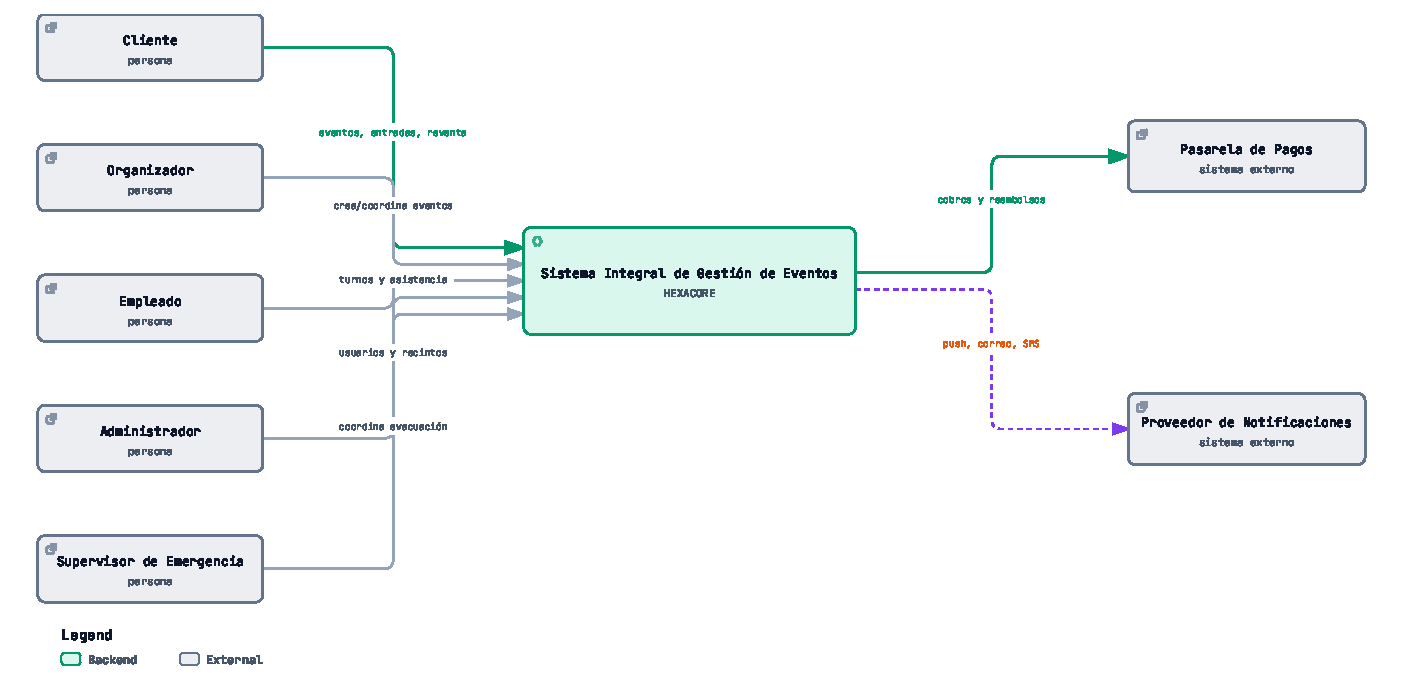
\includegraphics[height=0.66\textheight]{Diagrams/ArchifyPDF/01-contexto.pdf}
  \end{center}
  \footnotesize
  Cinco roles de usuario y \textbf{dos sistemas externos}: la pasarela de pagos y el proveedor de
  notificaciones. Ambos están fuera del alcance a propósito, y el sistema debe seguir siendo
  correcto cuando no respondan.
\end{frame}

\begin{frame}{Contenedores --- C4 nivel 2}
  \begin{center}
    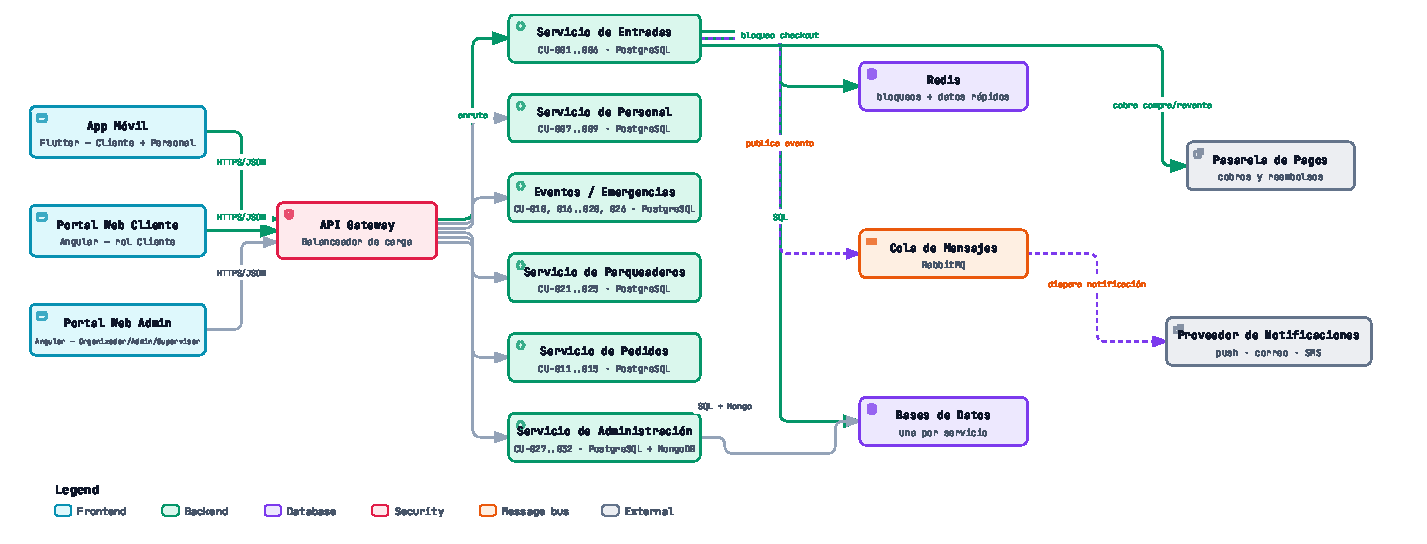
\includegraphics[height=0.66\textheight]{Diagrams/ArchifyPDF/02-contenedores.pdf}
  \end{center}
  \scriptsize
  \textbf{Tres interfaces} sobre un \textbf{único API Gateway} (ADR-02), que centraliza
  autenticación, autorización y enrutamiento. Detrás, microservicios por dominio con su propia
  base de datos, más Redis (bloqueo distribuido y datos de baja latencia) y RabbitMQ
  (operaciones asíncronas).
\end{frame}

\begin{frame}{Componentes --- Servicio de Entradas y Mercado Secundario}
  \begin{columns}[T]
    \begin{column}{0.58\textwidth}
      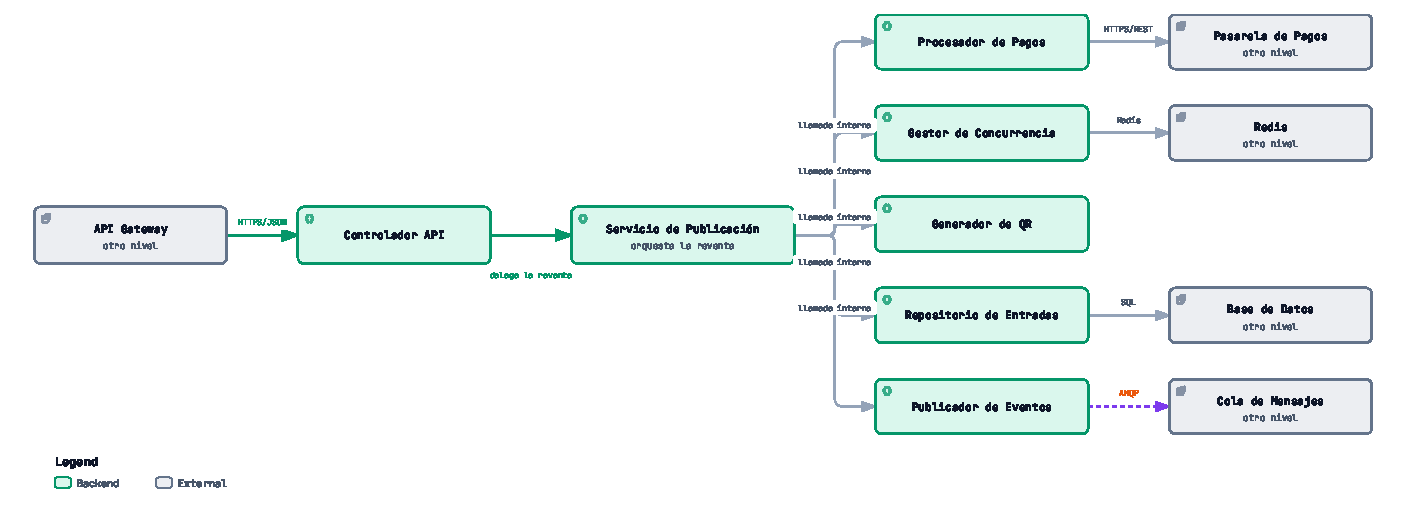
\includegraphics[width=\textwidth]{Diagrams/ArchifyPDF/03-componentes.pdf}
    \end{column}
    \begin{column}{0.40\textwidth}
      \scriptsize
      \textbf{El flujo de una reventa}
      \begin{enumerate}
        \item El \textbf{Controlador API} recibe lo que enrutó el Gateway.
        \item El \textbf{Servicio de Publicación} orquesta la operación.
        \item El \textbf{Gestor de Concurrencia} bloquea la entrada en Redis.
        \item El \textbf{Procesador de Pagos} cobra contra la pasarela.
        \item El \textbf{Generador de QR} invalida el código anterior y emite el nuevo.
        \item El \textbf{Repositorio} persiste el cambio de propiedad.
        \item El \textbf{Publicador de Eventos} avisa por la cola.
      \end{enumerate}
      \vspace{0.3em}
      Los otros tres servicios de dominio (Personal, Eventos/Emergencias, Parqueaderos) se
      documentan al mismo nivel en el SAD.
    \end{column}
  \end{columns}
\end{frame}

\begin{frame}{Procesos --- reventa de una entrada (CU-006)}
  \begin{columns}[T]
    \begin{column}{0.56\textwidth}
      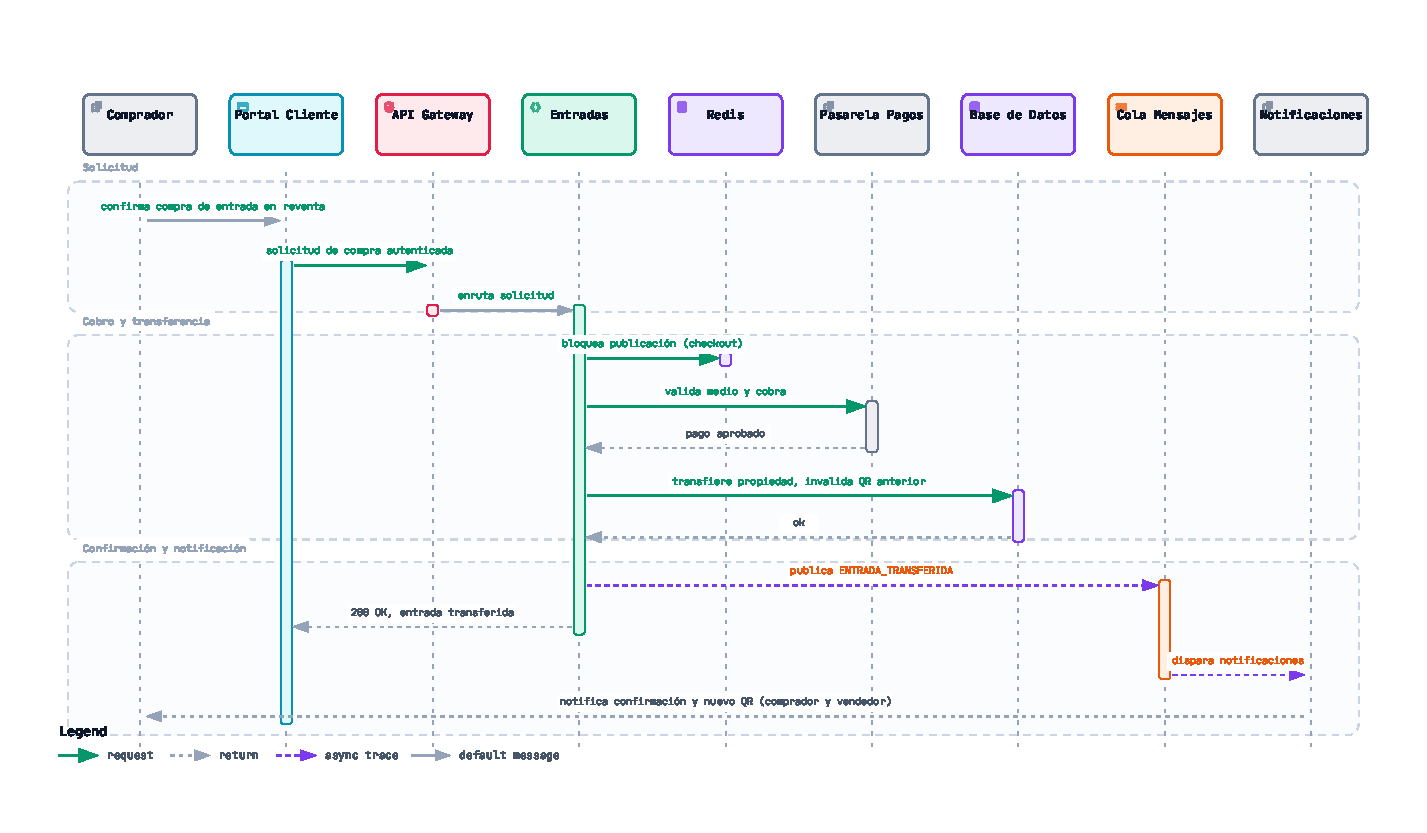
\includegraphics[width=\textwidth]{Diagrams/ArchifyPDF/05-secuencia.pdf}
    \end{column}
    \begin{column}{0.42\textwidth}
      \scriptsize
      \begin{enumerate}
        \item El comprador confirma la compra.
        \item El Gateway enruta la solicitud \textbf{ya autenticada}.
        \item Entradas \textbf{bloquea la publicación en Redis}: nadie más puede adquirirla.
        \item Se cobra por la pasarela de pagos.
        \item Se transfiere la propiedad y \textbf{se invalida el QR anterior}, en una sola
              transacción.
        \item Se publica \texttt{ENTRADA\_TRANSFERIDA} en la cola.
        \item Notificaciones envía el QR nuevo, desacoplado del flujo principal.
      \end{enumerate}
      \vspace{0.4em}
      \textbf{Evacuación (CU-010)} sigue el mismo patrón asíncrono: identificar zonas, confirmar
      protocolo, difundir por la cola y monitorear hasta el cierre.
    \end{column}
  \end{columns}
\end{frame}

\begin{frame}{Vista física --- producción, y lo que corre hoy}
  \begin{columns}[T]
    \begin{column}{0.56\textwidth}
      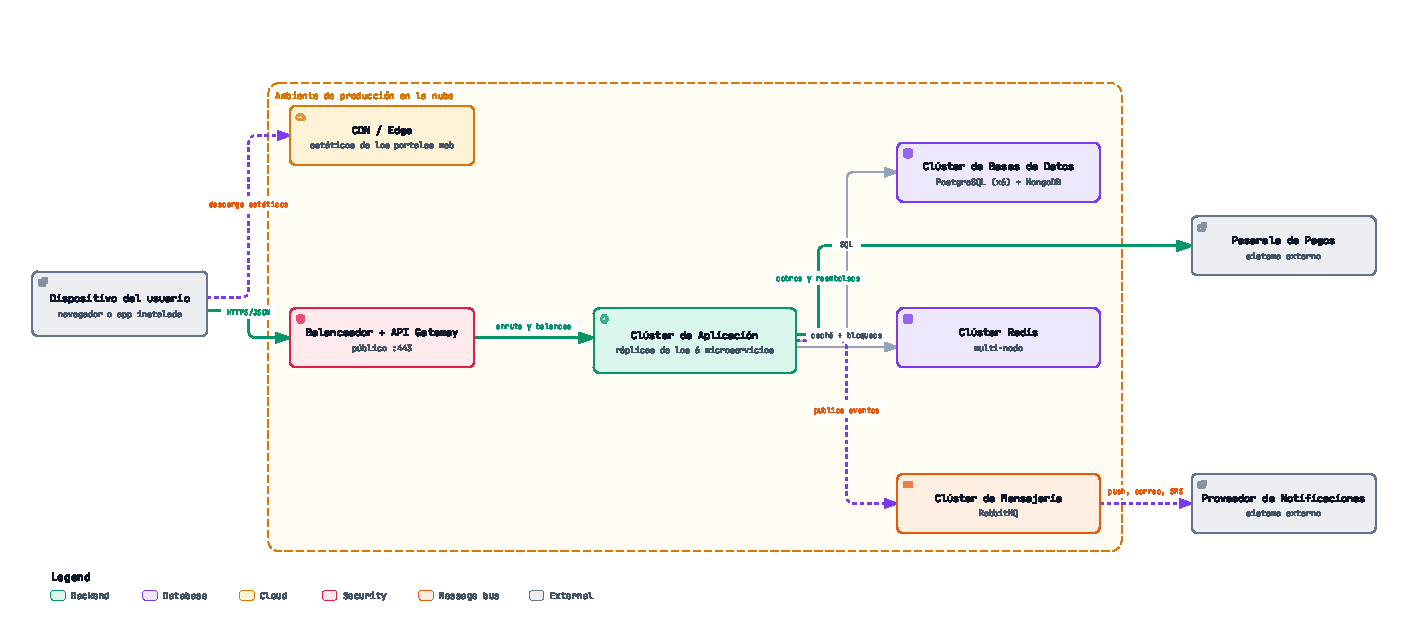
\includegraphics[width=\textwidth]{Diagrams/ArchifyPDF/06-despliegue.pdf}
    \end{column}
    \begin{column}{0.42\textwidth}
      \scriptsize
      \textbf{Producción} --- CDN para estáticos, balanceador + Gateway, clúster de aplicación con
      réplicas por microservicio, y clústeres de base de datos, Redis y mensajería.

      \vspace{0.5em}
      \textbf{Desarrollo y pruebas} --- misma topología a menor escala: una réplica por servicio,
      sin CDN, y Redis, cola y bases en un único nodo compartido.

      \vspace{0.5em}
      \begin{block}{Lo que se demuestra en vivo}
        El sistema repartido en \textbf{dos computadores}: la capa de datos en uno
        (\texttt{-{}-rol datos}) y los servicios más el Gateway en otro
        (\texttt{-{}-rol servicios -{}-datos <IP>}).
      \end{block}
    \end{column}
  \end{columns}
\end{frame}

\begin{frame}{Modelo de datos --- una base por microservicio}
  \scriptsize
  \begin{columns}[T]
    \begin{column}{0.5\textwidth}
      \textbf{Entradas / Mercado Secundario}
      \begin{itemize}\scriptsize
        \item \texttt{Entrada}(id, evento, localidad, \textbf{propietario}, codigoQR, estado)
        \item \texttt{PublicacionReventa}(id, entrada, vendedor, precio, estado)
        \item \texttt{TransaccionReventa}, \texttt{HistorialPropietario}, \texttt{Compra},
              \texttt{Ingreso}, \texttt{Cancelacion}
      \end{itemize}
      \textbf{Eventos / Emergencias}
      \begin{itemize}\scriptsize
        \item \texttt{Evento}, \texttt{Recinto}, \texttt{Zona}, \texttt{Incidente}
        \item \texttt{Turno}, \texttt{RegistroAsistencia}
      \end{itemize}
      \textbf{Pedidos}
      \begin{itemize}\scriptsize
        \item \texttt{Pedido}, \texttt{Establecimiento}, \texttt{Producto},
              \texttt{ReservaInventario}, \texttt{TransaccionPedido}
      \end{itemize}
    \end{column}
    \begin{column}{0.5\textwidth}
      \textbf{Administración}
      \begin{itemize}\scriptsize
        \item \texttt{Usuario}, \texttt{Rol}, \texttt{UsuarioRol}
        \item \texttt{Sesion}, \texttt{TokenCuenta}, \texttt{AuditoriaCuentas}
      \end{itemize}
      \vspace{0.6em}
      \begin{alertblock}{La regla que lo sostiene}
        \scriptsize Las referencias entre dominios se resuelven \textbf{en la aplicación}, con el
        identificador, y \textbf{no con llaves foráneas físicas} entre bases distintas. Es lo que
        permite que cada servicio evolucione y se despliegue solo (ADR-01).
      \end{alertblock}
      \vspace{0.3em}
      \scriptsize PostgreSQL para lo transaccional; MongoDB queda reservado para Reportes
      (ADR-06).
    \end{column}
  \end{columns}
\end{frame}

% =============================================================================
\section{Decisiones y riesgos}

\begin{frame}{Once decisiones arquitectónicas registradas}
  \scriptsize
  \begin{tabular}{C{1.1cm}L{4.6cm}L{6.6cm}}
    \toprule
    \textbf{ADR} & \textbf{Decisión} & \textbf{Por qué, y qué se descartó} \\
    \midrule
    ADR-01 & Microservicios por dominio & Escalar Entradas sin sobre-aprovisionar el resto;
      se descartó el monolito modular \\
    ADR-02 & API Gateway + balanceador & Un solo punto seguro de entrada; evita duplicar
      seguridad en tres interfaces \\
    ADR-03 & Redis para bloqueo y caché & Evita la doble venta sin volver la base el cuello de
      botella \\
    ADR-04 & Cola de mensajes asíncrona & Un fallo del proveedor externo no puede tumbar la
      compra \\
    ADR-05 & Angular en los portales & Módulos, guards e interceptors; trabajo en paralelo \\
    ADR-06 & PostgreSQL + MongoDB & ACID para lo transaccional; esquema flexible para reportes \\
    ADR-07 & Una sola app móvil para dos roles & El rol se resuelve en el login; menos
      configuración duplicada \\
    ADR-08 & Migración de la app a Flutter & ADR-05 omitió que la app debe llegar a Android
      \textbf{e iOS} \\
    \rowcolor{hexagris}
    ADR-09 & \textbf{NestJS} en el backend & Decidido con PoC medida, no por preferencia \\
    \rowcolor{hexagris}
    ADR-10 & \textbf{RabbitMQ} como cola & Decidido con PoC medida, no por popularidad \\
    ADR-11 & RS256 y dos tokens & Solo Administración firma; los demás solo verifican \\
    \bottomrule
  \end{tabular}
\end{frame}

\begin{frame}{Dos decisiones tomadas con evidencia, no con opinión}
  \scriptsize
  \begin{columns}[T]
    \begin{column}{0.5\textwidth}
      \textbf{ADR-09 --- Lenguaje del backend} \\[0.3em]
      Mismo endpoint en ambos, 100 conexiones, cero errores:
      \begin{tabular}{L{1.9cm}C{1.1cm}C{1.1cm}C{1.1cm}}
        \toprule
        & \textbf{req/s} & \textbf{p97,5} & \textbf{RSS} \\
        \midrule
        NestJS & 21.071 & 5 ms & 156 MB \\
        Spring Boot & \textbf{91.441} & 1 ms & 335 MB \\
        \bottomrule
      \end{tabular}
      \vspace{0.4em}

      \textbf{Spring Boot rinde 4,3$\times$ más}, y conviene decirlo sin matizarlo. Pero el umbral
      de RNF-07 es p95 $\leq$ 500 ms y el peor caso medido fue \textbf{7 ms}: setenta veces por
      debajo. \textbf{El rendimiento no decide.}

      Deciden Modificabilidad y Comprobabilidad ---NestJS impone el mismo modelo de módulos que
      el equipo ya usa en Angular--- y el cronograma: 4 personas, 6 servicios, un solo lenguaje
      entre frontend y backend.
    \end{column}
    \begin{column}{0.5\textwidth}
      \textbf{ADR-10 --- Motor de la cola} \\[0.3em]
      Evento real \texttt{ENTRADA\_TRANSFERIDA}, 500 mensajes:
      \begin{tabular}{L{2.2cm}C{1.3cm}C{1.3cm}}
        \toprule
        \textbf{Modo duradero} & \textbf{p50} & \textbf{p95} \\
        \midrule
        RabbitMQ & 162 ms & 282 ms \\
        Kafka & \textbf{31,6 ms} & \textbf{57,9 ms} \\
        \bottomrule
      \end{tabular}
      \vspace{0.4em}

      \textbf{Con durabilidad Kafka es cinco veces mejor.} Pero el umbral de RNF-17 es 10 s y el
      peor caso fue 282 ms: treinta y cinco veces por debajo. Otra vez, la latencia no decide.

      Decide el uso: esto es una \textbf{cola de tareas}, no un registro de eventos con
      reproducción histórica. RabbitMQ trae \textbf{DLQ y reintentos nativos} ---que ASR-07 y
      ASR-13 exigen--- con la mitad de memoria y de configuración.
    \end{column}
  \end{columns}
\end{frame}

\begin{frame}{Riesgos técnicos y su mitigación}
  \scriptsize
  \begin{tabular}{L{3.5cm}C{1.5cm}L{3.9cm}L{3.9cm}}
    \toprule
    \textbf{Riesgo} & \textbf{Prioridad} & \textbf{Mitigación} & \textbf{Contingencia} \\
    \midrule
    Concurrencia entre compradores en el mercado secundario & \textbf{Alta} &
      Bloqueo distribuido con TTL en Redis antes de pagar &
      Rechazar la segunda y notificar de inmediato \\
    Caída del API Gateway como punto único & \textbf{Alta} &
      Varias instancias, balanceador y \textit{health checks} &
      Failover hacia instancia o región de respaldo \\
    Indisponibilidad de la pasarela de pagos & \textbf{Alta} &
      Timeouts, reintentos y cola de reconciliación &
      Marcar pendiente y permitir reintento manual \\
    Picos en apertura de venta o ingreso masivo & \textbf{Alta} &
      Autoescalado de Entradas y caché en Redis &
      Sala de espera virtual que limita la concurrencia \\
    Fallo de notificaciones en una emergencia & Media &
      Reintentos y canal secundario (SMS si falla push) &
      Escalar el aviso mediante el personal en sitio \\
    Pérdida de conexión móvil durante una evacuación & Media &
      Caché local de instrucciones y reconexión &
      El personal de seguridad releva la comunicación \\
    \bottomrule
  \end{tabular}
\end{frame}

% =============================================================================
\section{Bitácora arquitectónica}

\begin{frame}{Cómo se registró el camino, no solo el resultado}
  \begin{columns}[T]
    \begin{column}{0.5\textwidth}
      \textbf{Bitácora grupal}
      \begin{itemize}\small
        \item \texttt{Documentation/Work/BitacoraArquitectonica.md}
        \item Registra \textbf{alternativas consideradas y descartadas}, no solo lo elegido:
              es de donde salieron los ADR.
        \item Incluye las dos pruebas de concepto medidas (PoC-04 lenguaje, PoC-05 cola) con sus
              datos crudos en \texttt{App/PoCs/}.
        \item Documenta las decisiones \textbf{revertidas}: ADR-05 quedó parcialmente superado por
              ADR-08 al detectar que la app debía llegar también a iOS.
      \end{itemize}
    \end{column}
    \begin{column}{0.5\textwidth}
      \textbf{Bitácora individual}
      \begin{itemize}\small
        \item Cada integrante lleva la suya sobre los casos de uso que le tocaron.
        \item El historial de Git la respalda: ramas
              \texttt{feature/<nombre>} y \textbf{pull request con revisión} obligatorio hacia
              \texttt{develop}.
      \end{itemize}
      \vspace{0.5em}
      \begin{block}{Trazabilidad viva}
        \small Los mensajes de commit explican \textbf{el problema, la solución y cómo se
        verificó}, de modo que la bitácora no es un documento aparte que se desincroniza sino
        el propio historial del repositorio.
      \end{block}
    \end{column}
  \end{columns}
\end{frame}

% =============================================================================
\section{Prototipo funcional}

\begin{frame}{Qué significa aquí ``implementado''}
  \begin{block}{Un caso de uso cuenta como completo solo si es end-to-end}
    GUI \ding{225} backend \ding{225} base de datos \ding{225} servicios de apoyo
    (Redis, RabbitMQ, pasarela de pagos), \textbf{y} con pruebas de integración que lo ejerciten
    por HTTP contra el sistema real.
  \end{block}

  \vspace{0.5em}
  \begin{columns}[T]
    \begin{column}{0.5\textwidth}
      \textbf{Lo que está desplegado y corriendo}
      \begin{itemize}\small
        \item \textbf{4 microservicios} NestJS con base propia
        \item \textbf{API Gateway} Nginx con \texttt{auth\_request}
        \item \textbf{2 portales} Angular + \textbf{app móvil} Flutter
        \item PostgreSQL, Redis, RabbitMQ
        \item Pasarela de pagos y correo simulados
      \end{itemize}
    \end{column}
    \begin{column}{0.5\textwidth}
      \textbf{La dependencia transversal, resuelta}
      \begin{itemize}\small
        \item \textbf{CU-027 (Autenticación)} está completo: registro, verificación por correo,
              login, renovación, recuperación y cierre de sesión.
        \item Es la que habilita a todas las demás: sin ella, ningún CU de Cliente o de Personal
              puede demostrarse.
      \end{itemize}
    \end{column}
  \end{columns}
\end{frame}

\begin{frame}{Estado por integrante --- casos de uso complejos}
  \scriptsize
  \begin{tabular}{L{2.4cm}C{1.5cm}L{4.5cm}C{1.1cm}C{1.1cm}C{1.1cm}C{1.3cm}}
    \toprule
    \textbf{Integrante} & \textbf{CU} & \textbf{Caso de uso} & \textbf{GUI} & \textbf{API} &
    \textbf{BD} & \textbf{Pruebas} \\
    \midrule
    \rowcolor{hexagris}
    \textbf{Samuel} & CU-006 & Mercado secundario \textit{(complejo)} & \ok & \ok & \ok & \ok \\
    Emperador & CU-026 & Gestión de eventos (CRUD) & \parcial & \ok & \ok & \ok \\
     & CU-007--010 & Personal y evacuación & \pend & \pend & \pend & \pend \\
     & CU-024--025 & Parqueadero: cobro y ocupación & \parcial & \pend & \pend & \pend \\
    \midrule
    \rowcolor{hexagris}
    \textbf{Daniel} & CU-001--005 & Boletería completa & \ok & \ok & \ok & \ok \\
    Cristancho & CU-021--023 & Parqueadero: reservas y accesos & \parcial & \pend & \pend & \pend \\
    \midrule
    \rowcolor{hexagris}
    \textbf{Sebastián} & CU-027 & Cuentas y autenticación & \ok & \ok & \ok & \ok \\
    Sánchez & CU-011--012 & Pedidos y menú & \ok & \ok & \ok & \ok \\
     & CU-013--015 & Preparación y entrega & \parcial & \parcial & \ok & \pend \\
     & CU-028--029 & Roles y recintos & \pend & \pend & \pend & \pend \\
    \midrule
    \rowcolor{hexagris}
    \textbf{Diego} & CU-017--018 & Personal operativo, turnos y asistencia & \ok & \ok & \ok & \ok \\
    Coronado & CU-019 & Monitoreo del evento & \parcial & \parcial & \ok & \parcial \\
     & CU-016, 020 & Logística e incidentes & \pend & \pend & \pend & \pend \\
     & CU-030--032 & Proveedores, pagos y reportes & \pend & \pend & \pend & \pend \\
    \bottomrule
  \end{tabular}

  \vspace{0.5em}
  \footnotesize
  \ok~completo \quad \parcial~parcial \quad \pend~no implementado
\end{frame}

\begin{frame}{CU-006 --- Mercado secundario, el caso complejo end-to-end}
  \scriptsize
  \begin{columns}[T]
    \begin{column}{0.52\textwidth}
      \textbf{Lo que ejercita una sola compra}
      \begin{itemize}\scriptsize
        \item \textbf{GUI:} portal web (mercado y ``mis entradas'') y app móvil
        \item \textbf{Gateway:} valida el token antes de enrutar
        \item \textbf{Redis:} bloqueo del checkout con dueño y TTL
        \item \textbf{PostgreSQL:} transferencia de propiedad, QR nuevo e historial, en
              \textbf{una sola transacción}
        \item \textbf{Pasarela:} cobro con clave de idempotencia
        \item \textbf{RabbitMQ:} \texttt{ENTRADA\_TRANSFERIDA} hacia notificaciones y liquidación
      \end{itemize}
      \vspace{0.4em}
      \textbf{Caminos alternos cubiertos por pruebas} \\
      CU-006A cambio de precio · CU-006B retiro · CU-006D expiración ·
      CU-006E entrada no revendible · CU-006F evento sin reventa ·
      CU-006G pago rechazado · CU-006H compra simultánea · CU-006I pasarela caída
    \end{column}
    \begin{column}{0.46\textwidth}
      \begin{block}{Post-condiciones verificadas contra la base}
        \scriptsize
        \begin{itemize}
          \item La propiedad cambió al comprador
          \item El QR anterior \textbf{no existe en ninguna fila} (RNF-02)
          \item El historial queda \texttt{EMISION} $\rightarrow$ \texttt{REVENTA} (RNF-11)
          \item El reparto cuadra al céntimo:
                \texttt{precio = comisión + neto}
        \end{itemize}
      \end{block}
      \vspace{0.3em}
      \begin{alertblock}{Lo que el historial no admite}
        \scriptsize Un disparador rechaza \texttt{UPDATE} y \texttt{DELETE} sobre
        \texttt{historial\_propietarios}: la cadena de propiedad no se puede reescribir desde la
        aplicación.
      \end{alertblock}
    \end{column}
  \end{columns}
\end{frame}

\begin{frame}{Cobertura de pruebas de integración sobre el backend}
  \begin{columns}[T]
    \begin{column}{0.54\textwidth}
      \begin{tikzpicture}
        \begin{axis}[
          width=\textwidth, height=5.2cm,
          xbar, xmin=0, xmax=100,
          bar width=11pt,
          symbolic y coords={Pedidos, Eventos/Emerg., Entradas, Administración},
          ytick=data, y dir=reverse,
          nodes near coords, nodes near coords style={font=\tiny},
          xlabel={\tiny \% de líneas cubiertas},
          tick label style={font=\tiny},
          every node near coord/.append style={xshift=1pt},
          enlarge y limits=0.25,
          grid=major, grid style={hexagris},
          axis lines*=left,
        ]
        \addplot[fill=hexaacento, draw=none] coordinates {
          (92.58,Pedidos) (91.37,Eventos/Emerg.) (94.03,Entradas) (94.95,Administración)};
        \end{axis}
      \end{tikzpicture}
      \vspace{-0.3em}
      \scriptsize
      \textbf{20 suites} de integración que hablan por HTTP contra el sistema real, más 59
      pruebas e2e en Eventos/Emergencias.
    \end{column}
    \begin{column}{0.44\textwidth}
      \scriptsize
      \begin{alertblock}{Por qué no es 100\,\%, dicho de frente}
        Lo que falta son \textbf{tres cosas distintas}:
        \begin{itemize}
          \item Rutas de fallo de infraestructura (Redis caído, canal de RabbitMQ cerrado) y
                validaciones que solo se disparan al arrancar mal. Llegar ahí pide
                \textbf{inyección de fallos}.
          \item Un \textbf{artefacto de medición} en los DTO: el plugin de Swagger genera en cada
                clase un método cuyo mapa de fuentes abarca todo el bloque de propiedades. Se ve a
                simple vista: hay \textbf{comentarios} marcados como no cubiertos.
        \end{itemize}
        No se excluyen los DTO para maquillar el porcentaje: esconderlos escondería también sus
        funciones de mapeo, que sí se prueban.
      \end{alertblock}
    \end{column}
  \end{columns}
\end{frame}

% =============================================================================
\section{Atributos de calidad}

\begin{frame}{Cinco atributos, medidos con una sola orden}
  \begin{block}{\texttt{cd App/infra \&\& ./atributos-calidad.py}}
    \small Corre las cuatro suites \textbf{contra el sistema desplegado} ---a través del
    Gateway, por donde entra el tráfico real--- y deja el informe escrito en
    \texttt{informe-atributos/INFORME.md}.
  \end{block}

  \vspace{0.3em}
  \scriptsize
  \begin{tabular}{L{2.6cm}L{2.3cm}L{4.4cm}L{3.4cm}}
    \toprule
    \textbf{Atributo} & \textbf{RNF} & \textbf{Resultado} & \textbf{Referencia} \\
    \midrule
    Desempeño & RNF-07, 08 & \cifra{p95 189,9 ms} con 200 simultáneas; \cifra{0} fallidas &
      umbral 500 ms \\
    Disponibilidad & RNF-03, 04 & En pie \cifra{1,3 s} tras \texttt{kill -9} & exigido $\leq$ 30 s \\
    Seguridad & RNF-05, 06 & \cifra{11 de 11} rutas responden 401 sin token & exigido 0 \% abiertas \\
    Consistencia & RNF-01, 02 & \cifra{1} checkout y \cifra{49} rechazos con 50 compradores &
      exigido exactamente 1 \\
    Desplegabilidad & RNF-15 & \cifra{88 s} de cero a sistema utilizable & un solo guion \\
    \bottomrule
  \end{tabular}

  \vspace{0.4em}
  {\footnotesize Si una suite falla, su fila queda marcada como fallida y el guion termina con
  error: \textbf{no rellena el hueco con la cifra de la corrida anterior}.}
\end{frame}

\begin{frame}{Desempeño --- RNF-07 bajo carga creciente}
  \begin{columns}[T]
    \begin{column}{0.56\textwidth}
      \begin{tikzpicture}
        \begin{axis}[
          width=\textwidth, height=5.3cm,
          xlabel={\tiny peticiones simultáneas}, ylabel={\tiny p95 (ms)},
          xmode=log, log basis x=10,
          xtick={1,10,50,100,200}, xticklabels={1,10,50,100,200},
          tick label style={font=\tiny}, label style={font=\tiny},
          ymin=0, ymax=560,
          grid=major, grid style={hexagris},
          axis lines*=left,
          legend style={font=\tiny, at={(0.03,0.97)}, anchor=north west, draw=none},
        ]
        \addplot[hexapend, dashed, thick, no markers] coordinates {(1,500) (200,500)};
        \addlegendentry{umbral RNF-07}
        \addplot[hexaacento, thick, mark=*, mark size=1.6pt] coordinates {
          (1,5.3) (10,25.7) (50,101.3) (100,158.3) (200,262.4)};
        \addlegendentry{p95 medido}
        \end{axis}
      \end{tikzpicture}
    \end{column}
    \begin{column}{0.42\textwidth}
      \scriptsize
      \begin{tabular}{C{1.3cm}C{1.1cm}C{1.4cm}}
        \toprule
        \textbf{Simult.} & \textbf{p95} & \textbf{pet/s} \\
        \midrule
        1 & 5,3 ms & 253 \\
        10 & 25,7 ms & 630 \\
        50 & 101,3 ms & 693 \\
        100 & 158,3 ms & 735 \\
        \rowcolor{hexagris}
        200 & \textbf{262,4 ms} & \textbf{781} \\
        \bottomrule
      \end{tabular}
      \vspace{0.5em}

      Peor caso medido \cifra{262,4 ms} frente a un umbral de \textbf{500 ms}, con
      \cifra{0} peticiones fallidas en toda la prueba.

      \vspace{0.4em}
      Las tácticas detrás: caché con \texttt{Cache-Control} en la cartelera, réplicas tras el
      balanceador, resolución del destino \textbf{en cada petición}, y pool de conexiones acotado
      por servicio.
    \end{column}
  \end{columns}
\end{frame}

\begin{frame}{Consistencia --- RNF-01: cero ventas duplicadas}
  \scriptsize
  \begin{columns}[T]
    \begin{column}{0.47\textwidth}
      \begin{tabular}{L{3.6cm}C{2.5cm}}
        \toprule
        \textbf{Escenario} & \textbf{Resultado} \\
        \midrule
        50 compradores a la vez sobre la misma entrada & \cifra{1} checkout, \cifra{49} rechazados \\
        Pagar con la reserva ya caducada & \cifra{1} cobro aprobado \\
        Los dos pagan simultáneamente & \cifra{1} pago, \cifra{1} QR \\
        Dos puertas escanean el mismo QR & \cifra{1} ingreso; el aforo sube \cifra{1} \\
        \bottomrule
      \end{tabular}
      \vspace{0.6em}

      \textbf{Ocho tácticas} lo sostienen: bloqueo pesimista, escrituras condicionales que miran
      cuántas filas cambiaron, bloqueo distribuido con dueño, claves de idempotencia, invariantes
      en la propia base, una sola transacción por transferencia, historial inmutable y el orden
      anular-antes-de-reembolsar.
    \end{column}
    \begin{column}{0.51\textwidth}
      \begin{block}{La red que queda si la lógica fallara}
        \scriptsize
        Invariantes que \textbf{la base de datos} no admitiría violar:
        \begin{itemize}
          \item Índice único parcial: \textbf{una sola publicación activa} por entrada
          \item \texttt{UNIQUE} sobre \texttt{ingresos.entrada\_id}: un QR no ingresa dos veces
          \item \texttt{CHECK}: \texttt{precio = comisión + neto}
          \item \texttt{CHECK}: una transacción aprobada \textbf{exige} referencia de la pasarela
        \end{itemize}
      \end{block}
      \vspace{0.3em}
      \begin{alertblock}{Por qué importa el orden}
        \scriptsize En la cancelación se \textbf{anula primero y se reembolsa después}: así la
        entrada no se puede usar en la puerta mientras el dinero está en vuelo. Si la pasarela
        rechaza, las entradas vuelven a ser válidas.
      \end{alertblock}
    \end{column}
  \end{columns}
\end{frame}

\begin{frame}{Seguridad y disponibilidad --- RNF-03 a RNF-06}
  \scriptsize
  \begin{columns}[T]
    \begin{column}{0.5\textwidth}
      \textbf{Seguridad (RNF-06)}
      \begin{tabular}{L{3.4cm}C{2.3cm}}
        \toprule
        \textbf{Comprobación} & \textbf{Resultado} \\
        \midrule
        Rutas de negocio sin token & \cifra{11 de 11} dan 401 \\
        Formas de token inválido & \cifra{8} rechazadas \\
        Revocación al cerrar sesión & \cifra{inmediata} \\
        Si Redis no responde & \cifra{503}, no se entra \\
        \bottomrule
      \end{tabular}
      \vspace{0.4em}

      Se rechazan token firmado con otra clave, \texttt{alg: none}, \texttt{HS256} usando la clave
      pública como secreto, caducado, de otro emisor y manipulado.

      \vspace{0.3em}
      \textbf{RNF-05:} de los pagos solo se guarda una \textbf{referencia opaca}. Ni el esquema ni
      los eventos publicados tienen campo para número de tarjeta.
    \end{column}
    \begin{column}{0.48\textwidth}
      \textbf{Disponibilidad (RNF-03, RNF-04)}
      \begin{tabular}{L{3.2cm}C{2.5cm}}
        \toprule
        \textbf{Dependencia caída} & \textbf{El login} \\
        \midrule
        Redis & \cifra{200} en 90 ms \\
        RabbitMQ & \cifra{200} en 95 ms \\
        PostgreSQL & \cifra{503} honesto \\
        \midrule
        \texttt{kill -9} del proceso & en pie en \cifra{1,3 s} \\
        \bottomrule
      \end{tabular}
      \vspace{0.5em}

      \begin{block}{Fallar en claro también es disponibilidad}
        \scriptsize Sin base de datos \textbf{no hay login posible}. Lo que se exige entonces no es
        un 200 falso, sino un \textbf{503 rápido} que un balanceador entienda como ``prueba otra
        instancia'' ---y que \texttt{/salud} lo diga.
      \end{block}
    \end{column}
  \end{columns}
\end{frame}

\begin{frame}{Desplegabilidad --- dos computadores, un solo guion}
  \begin{columns}[T]
    \begin{column}{0.5\textwidth}
      \scriptsize
      \textbf{Un único guion levanta el sistema completo}
      \begin{block}{\texttt{cd App/infra \&\& ./iniciar.sh}}
        \scriptsize De cero a sistema \textbf{utilizable} en \cifra{88 s}: levanta la
        infraestructura, aplica las migraciones, siembra los datos y prepara el inventario en
        Redis.
      \end{block}
      \vspace{0.4em}
      \textbf{Repartido en dos máquinas}
      \begin{itemize}\scriptsize
        \item Computador A: \texttt{./iniciar.sh -{}-rol datos}
        \item Computador B: \texttt{./iniciar.sh -{}-rol servicios -{}-datos <IP>}
      \end{itemize}
      \vspace{0.3em}
      \scriptsize
      Verificado: en la máquina de servicios arrancan \cifra{6} contenedores ---los 4 servicios,
      el Gateway y el portal--- y \textbf{ninguno} de la capa de datos.
    \end{column}
    \begin{column}{0.48\textwidth}
      \scriptsize
      \textbf{Otras opciones del mismo guion}
      \begin{itemize}\scriptsize
        \item \texttt{-{}-replicas 2} --- varias instancias de Entradas tras el balanceador
        \item \texttt{-{}-registro develop} --- despliega \textbf{sin código fuente}, desde las
              imágenes que publicó el pipeline
        \item \texttt{-{}-datos-demo sql} --- datos de ejemplo sin necesitar Node
      \end{itemize}
      \vspace{0.5em}
      \begin{alertblock}{Despliegue sin compilar nada}
        \scriptsize Una máquina con \textbf{solo Docker} levanta el sistema con datos usables:
        se bajan las siete imágenes ya construidas y se levantan. La diferencia es de minutos a
        segundos.
      \end{alertblock}
    \end{column}
  \end{columns}
\end{frame}

\begin{frame}{El pipeline CI/CD}
  \scriptsize
  \begin{columns}[T]
    \begin{column}{0.5\textwidth}
      \textbf{Integración continua} --- en cada pull request
      \begin{itemize}\scriptsize
        \item Guardia de \textbf{artefactos versionados} (nada de \texttt{dist/} ni
              \texttt{node\_modules/})
        \item Chequeo de tipos, pruebas unitarias y compilación de los \textbf{4 servicios}
        \item Compilación de los \textbf{2 portales} Angular
        \item Análisis estático y pruebas de widget de la \textbf{app Flutter}
        \item Validación del \texttt{nginx.conf} y de los \texttt{docker-compose}
        \item \textbf{Pruebas de integración}: levanta el sistema con
              \texttt{./iniciar.sh} y corre las 20 suites
      \end{itemize}
    \end{column}
    \begin{column}{0.48\textwidth}
      \textbf{Entrega continua} --- en cada merge a \texttt{develop} o \texttt{main}
      \begin{itemize}\scriptsize
        \item Construye y publica \textbf{7 imágenes} multi-arquitectura
              (\texttt{amd64} y \texttt{arm64}) en \texttt{ghcr.io}
        \item Tres etiquetas por imagen: la rama, el \textbf{commit exacto}
              (\texttt{sha-XXXXXXX}) y \texttt{latest}
        \item Un trabajo final \textbf{baja lo publicado y comprueba que arranca}
      \end{itemize}
      \vspace{0.4em}
      \begin{block}{El guion de arranque, integrado al pipeline}
        \scriptsize El trabajo de integración usa \textbf{el mismo \texttt{iniciar.sh} de la
        demostración}. Así el guion queda probado en cada PR, no solo el día de la entrega.
      \end{block}
    \end{column}
  \end{columns}
\end{frame}

% =============================================================================
\section{Cierre}

\begin{frame}{Dónde estamos}
  \begin{columns}[T]
    \begin{column}{0.5\textwidth}
      \textbf{Entregado y verificable}
      \begin{itemize}\small
        \item SRS completo (IEEE 830) y SAD con las 15 secciones del formato
        \item \textbf{CU-006} (complejo) end-to-end, con sus 8 caminos alternos
        \item CU-001--005, CU-011--012, CU-017--018 y CU-027 end-to-end
        \item \textbf{5 atributos} de calidad con cifras reproducibles en una orden
        \item Sistema repartible en \textbf{2 computadores} desde un guion
        \item CI/CD con pruebas de integración y 7 imágenes publicadas
      \end{itemize}
    \end{column}
    \begin{column}{0.48\textwidth}
      \textbf{Lo que falta, sin adornos}
      \begin{itemize}\small
        \item \textbf{CU-010 (evacuación)}, el segundo caso complejo, sin implementar
        \item Parqueaderos (CU-021--025) sin backend
        \item Personal propio (CU-007--009) sin backend
        \item Proveedores, pagos y reportes (CU-030--032) en placeholder
        \item La cobertura de integración está en \textbf{91--95\,\%}, no en 100\,\%
      \end{itemize}
      \vspace{0.4em}
      \begin{alertblock}{}
        \small Preferimos decir qué falta a presentar como terminado algo que no lo está.
      \end{alertblock}
    \end{column}
  \end{columns}
\end{frame}

\begin{frame}[standout]
  Gracias \\[0.5em]
  \small Demostración en vivo a continuación
\end{frame}

\end{document}
